\section{Broader Impacts}
\label{sec:broader-impacts}

We highlight below two activities designed to broaden the project's impacts: contributions to three undergraduate internship programs dedicated to improving diversity, equity, and inclusion in the geosciences, and development of a novel web-accessible simulation that integrates models to provide a dynamic visualization of an evolving micro-continent. In terms of other broad impacts, the student summer program will provide 12 graduate students with computational experience, assisted by professional research software engineers; it will also provide these students an opportunity to widen their professional networks. The project also provides support for graduate students at the collaborating universities.

\subsection{Promoting Diversity in Geosciences}
\label{sec:promoting-diversity}

The geosciences are among the least diverse STEM disciplines. Among the many contributing factors is lack of access to meaningful research opportunities, at the undergraduate level, especially in 2-year colleges and minority-serving institutions. A further contributing factor may be lack of awareness among many students, especially from traditionally under-served backgrounds of the high value of scientific computing skills in the broader job market \citep{bernard2018no}. In the spirit of leveraging existing programs, we propose to contribute to addressing these issues by partnering with three summer research internship programs for undergraduate students: RESESS, a summer internship program dedicated to increasing the diversity of students entering the geosciences; RECCS, which gives community college students an authentic research experience in geosciences; and SOARS, an undergraduate-to-graduate bridge program designed to broaden participation of historically underrepresented communities in the atmospheric and related sciences. We will work with the RESESS and RECCS teams to design and implement computational science workshops, with the aim of equipping interns with computational thinking skills and basic scientific programming in Python. The workshops will combine hands-on instruction with self-paced online learning resources, and available help from a research software engineer. SOARS already offers a computational component, so the project's contribution to their program will center on  contributing curricular material that illustrates applications of computer modeling in the surface-Earth and solid-Earth sciences, including various community tools and models.


\begin{wrapfigure}{R}{0.32\textwidth}
  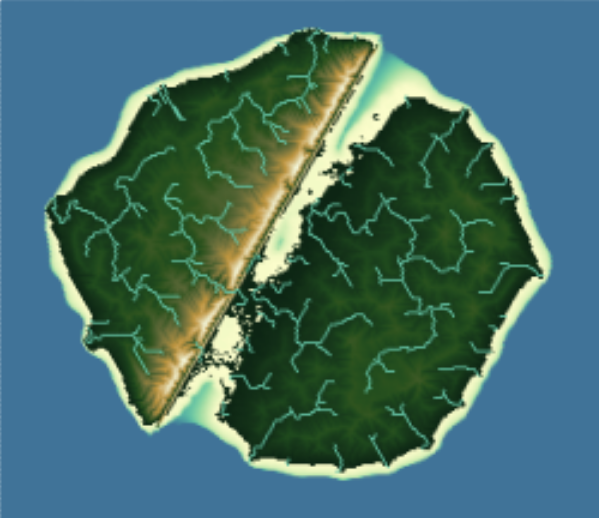
\includegraphics[width=0.32\textwidth]{island_world.png}
  \caption{Prototype OpenEarthscape Simulator, viewed from above, showing hypothetical ocean microcontinent undergoing active rifting.}% Stochastic variations in sea level influence accumulation and dispersal of sediment around island margins.}
  \label{fig:islandworld}
\end{wrapfigure}

\subsection{OpenEarthscape Simulator}
\label{sec:oes}

One barrier to widespread public appreciation of geosciences is the difficulty in conceptualizing dynamics that play out across such a wide spectrum of space and time scales. Media present geologic events with a lens that rarely encompasses larger context.
Visualization is a great way to present this context. To that end, we will create the OpenEarthscape Simulator: a dynamic, web-visualized simulation of the ongoing evolution of a hypothetical micro-continental island (Fig.~\ref{fig:islandworld}). Randomly generated climatic, volcanic, sea-level, and tectonic events will drive the simulation. The web app will display the latest stage in the island's configuration, so that viewers can observe its evolution slowly unfold over time. Viewers will be able to zoom in/out, and the 3D rendering will update periodically as the system evolves. The website will include links to resources for learning more about the processes, and to time-lapse images of real geologic situations (meandering rivers, migrating barrier islands, etc.). %Target audiences for the Simulator include Earth science classes and curious members of the general public.

\section{Outcomes, Metrics, and Sustainability}

\subsection{Project Management}

The project will be managed by the lead PI, in close consultation with the collaborating PIs. A Scientific Steering Committee (SSC) will be formed in Year 1 to provide high-level guidance. Details on the approach to coordination and integration are provided in the \textit{Management and Coordination Plan}, as are year-by-year goals.

%\subsection{Anticipated Outcomes and Deliverables}

%This project will create OpenEarthscape as an open-source collection of tools, libraries, standards, and resources. The OpenEarthscape suite will be hosted on the CSDMS web portal (csdms.colorado.edu), with overview documentation and pointers to each element. Documentation for each product will be developed using Sphinx. Sources for products, docs, and tutorials will be hosted on GitHub. Tutorials will take the form of Jupyter Notebooks, and will be accessible and operable via the OpenEarthscape JupyterHubs as well as being available for direct download. This includes tutorials arising from science demonstration projects.

%We may need to ditch this section for space, or modify... somehow however need to make it clear to reviewers what the deliverables/products are, in summary fashion. Maybe summarize as a collection of tools and resources under the heading OpenEarthscape, hung off of CSDMS website.

%[*This relatively short section addresses RC 6. Deliverables, by providing a summary/list of major project deliverables*]

\subsection{Metrics and Deliverables}

\textbf{Metrics:} We divide our Metrics of Success into four categories: Awareness, Usage and Adoption, Tool Development, and Training. OpenEarthscape will implement a strategy of continual monitoring and adaption of the identified metrics, with annual metric reporting to the Steering Committee. In addition, OpenEarthscape will present results of feedback and metrics at a Science Gateways Community Institute (SGCI) Annual Meeting. Metrics are detailed in the supplemental document \textit{Delivery Mechanism and Community Usage Metrics.}

\scitem{Deliverables:} This project will create OpenEarthscape as an open-source collection of tools, libraries, standards, and resources. %The OpenEarthscape suite will be hosted on the CSDMS web portal (csdms.colorado.edu), with overview documentation and pointers to each element.
Documentation for each product will be developed using Sphinx. Sources for products, docs, and tutorials will be hosted on GitHub. Tutorials, including those arising from science demonstration projects, will take the form of Jupyter Notebooks, and be accessible and operable via the OpenEarthscape JupyterHub. For further details see the \textit{Data Management Plan} and \textit{Delivery Mechanism and Community Usage Metrics}.




\subsection{Sustained and Sustainable Impacts}

 Here we describe planned practices intended to sustain the created cyberinfrastructure beyond the funding lifetime of the proposed research.
Sustainability of the two Python packages (PyMT and Landlab) will be accomplished through software development best practices and continuing to nurture the user base. Our sustainability plan for the code base is driven by a design principle to create software that reduces sustainability overhead. Importantly, each of the packages already exists and has a user base. By improving the packages and developing trainings, we further support and grow the user base. Both packages currently employ software development best practices including: (1) open source licensing; (2) version control; (3) use of development/release branches; (4) integrated test suite; (5) testing of cross-platform distribution using continuous integration, PyPI, and conda-forge; (6) integrated documentation through docstrings, and (7) the creation of a user knowledge base through publicly accessible and searchable GitHub issues. Further, the proposed work improves the scalability of PyMT and Landlab.


\subsubsection{The OpenEarthscape Software Council}
\label{sec:software-council}

Software products such as BMI, Babelizer, CSN, and PyMT originated as CSDMS projects, and, along with Landlab, CSDMS staff have been responsible for their development and upkeep.
However, groups outside of CSDMS use these products, and contribute their ideas and efforts to their development.
Since all of these products are open source, and they were designed with community support in mind, these groups should have a say in guiding their development.
To this end, we propose to create the \textbf{OpenEarthscape Software Council} to represent the interests of all users of these software products.
We have obtained letters of collaboration from researchers at Deltares, Netherlands eScience Center, and the USGS, who are willing to serve on the Council.

\subsection*{Results from Prior NSF Support}

\noindent
\emph{\underline{Tucker, Gasparini, Istanbulluoglu}}: SI2-SSI (ACI-1450409) ``Collaborative Research: SI2-SSI: Landlab: a flexible, open-source modeling framework for earth-surface dynamics'' (\$787,846, 8/2015--7/2020).
\textbf{Intellectual Merit:} Project applied new modeling tools to research problems in geomorphology, hydrology, and geohazards. \textbf{Broader Impacts:} Outreach activities included training workshops, online user support, site visits, and documentation. \textbf{Publications \& Products:} The project created Landlab 2.0 and associated tutorials and documentation, and produced 25 peer-reviewed publications to date (listed in References).

\noindent
\emph{\underline{Hutton, Kettner, Overeem, Tucker}}: (EAR-1831623) ``Community Facility Support: The Community Surface Dynamics Modeling System'' (\$3.6M, 10/2018--9/2021).
\textbf{Intellectual Merit}: CSDMS is a community-driven program that seeks to transform the science and practice of  earth-surface dynamics modeling, with a focus on model coupling and  best practices in software development.
\textbf{Broader Impacts}:  Organized, hosted, or sponsored 13 workshops \& meetings, 6 short courses, 16 webinars, a summer science series, and the Earth Surface Processes Institute (ESPIn). CSDMS is a diverse community of 1985 members representing nearly 200 US institutions and $>$300 non-US institutions from 73 countries.
\textbf{Publications}: 21 peer-reviewed publications to date from CSDMS staff and community members using CSDMS products (listed in References).
\textbf{Products}: The CSDMS EKT Repository hosts 18 training labs, 81 animations and 9 lectures. The Model Repository hosts 383 open source codes. CSDMS staff develop and maintain  CSDMS Workbench. %consisting of the Python Modeling Tool (pymt), Landlab, the Basic Model Interface (BMI), CSDMS Standard Names, babelizer, bmi-tester, dakotathon, and the Permafrost Benchmark System.

